\section{Introduction}
Recent advances in biomedical image analysis have assisted many pathologists and biologists to facilitate their researches \cite{Chen2016b,Ronneberger2015,Chen2016c,Lieman-Sifry2017,Paszke2016,Tseng2017,Sirinukunwattana2015b}.
Among these researches, a significant application is to obtain the accurate segmentation of specific membrane objects in a biomedical image, such as lumenal glands, synaptic vesicles and cells.
The morphological shape and spatial distribution of synaptic vesicles are helpful to study the neural activity in different brain regions, while morphological statistics of lumenal glands are widely used for assessment of the malignancy degree of adenocarcinomas.
Conventionally, these crucial steps are performed by human expert, which are time-consuming and suffer from subjective factors.
Therefore, it is significantly demanded to improve the efficiency as well as the reliability with automatic segmentation methods.

\begin{figure}
    \begin{center}
        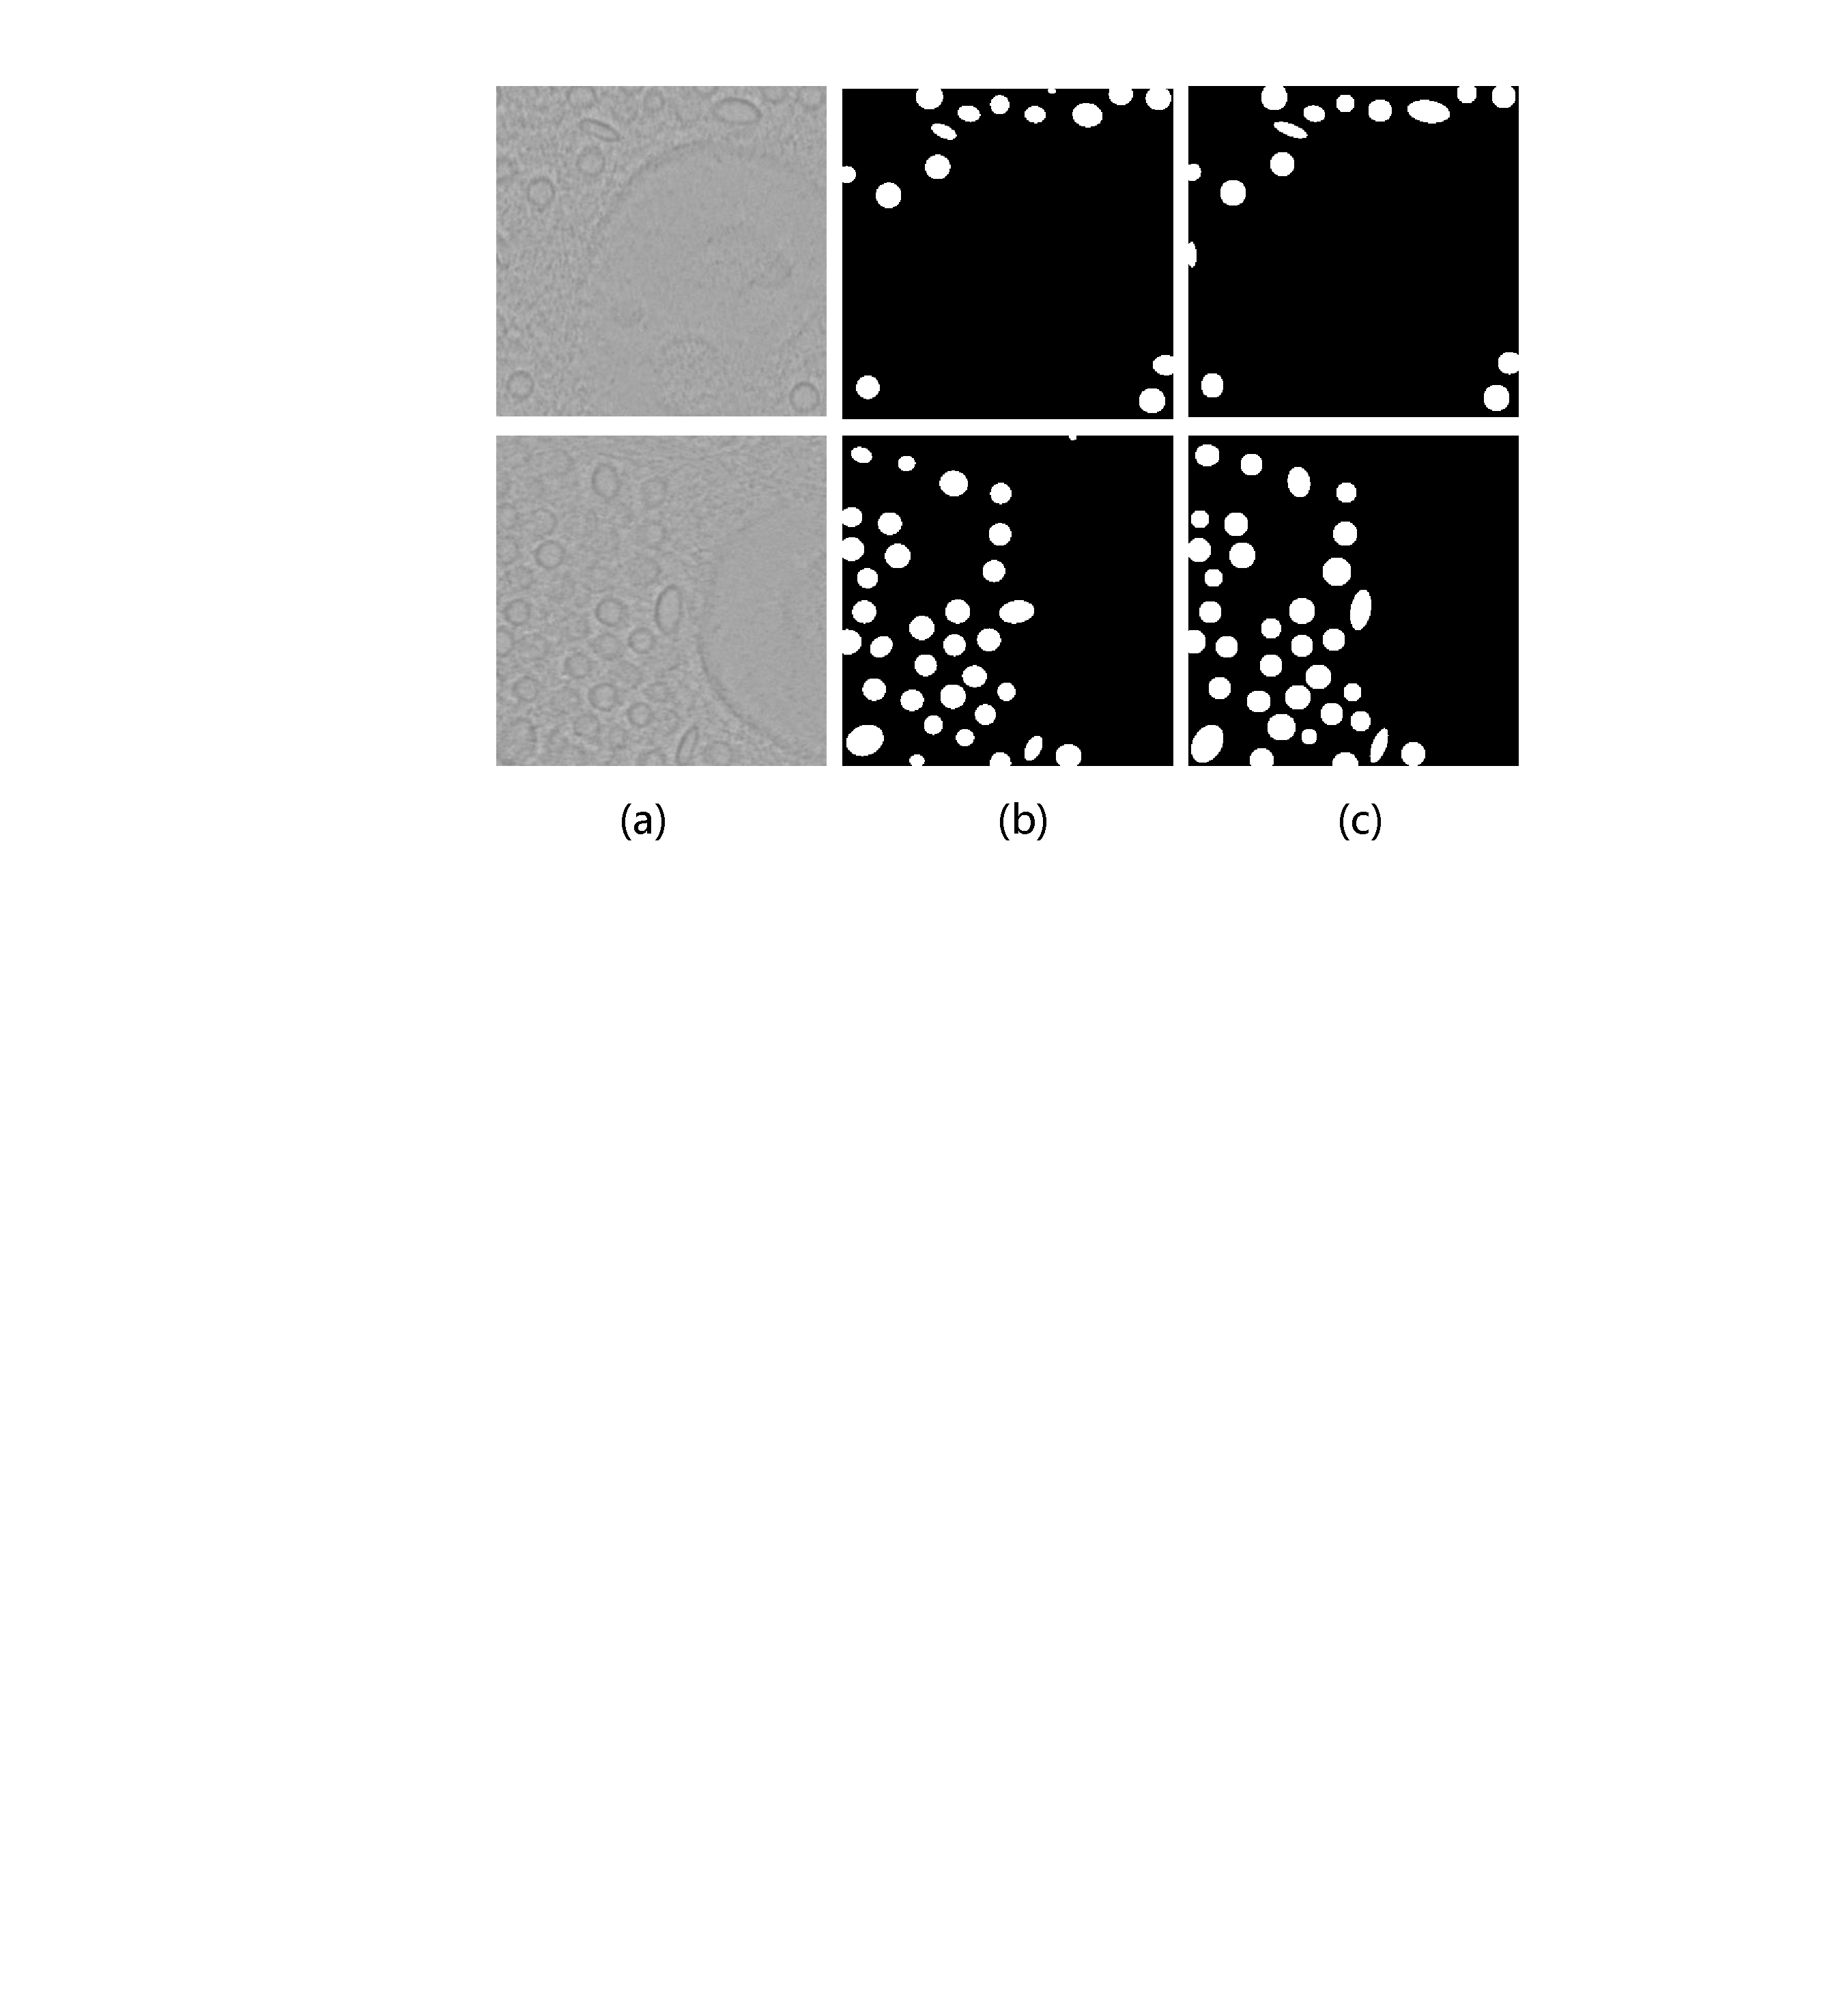
\includegraphics[width=3.3in]{figures/FigImg.pdf}
    \end{center}
    \caption{Examples of challenging biomedical segmentation: (a) biomedical image; (b) results from proposed DSAN by incorporating prior shape knowledge; (c) annotations by experts.}
    \label{FigImgs}
\end{figure}

However, it is non-trivial to automatically segment objects in biomedical images.
First, biomedical images are usually noisy and ambiguous caused by deficient imaging techniques, as shown in Figure~\ref{FigImgs} (a).
Second, the dense arrangement and blurry boundaries of objects in biomedical images make it hard to separate adjacent objects individually, which is known as the touching problem.
Finally it is challenging to incorporate prior shape knowledge about plausible objects to into the model, because of huge variation of some pathological objects, \cite{Sirinukunwattana2015b}.

Recently, fully convolution network (FCN) networks have shown tremendous progress in image segmentation \cite{Long2015a,Chen2016d,Dai2015,Zheng2015}.
The famous U-shaped deep network called U-net~\cite{Ronneberger2015} was proposed for biomedical image segmentation, which obtained great performance in solving touching problem.
To solve the touching problem, the U-net used skip connections between contracting and expanding paths to supplement the lost information and further added weighting losses on boundary pixels for clear boundaries in segmentation.
Soon, DeepVentricle~\cite{Lieman-Sifry2017} uses the same padding instead of valid padding in cardiac segmentation and Chen et al. \cite{Chen2016c} proposed kU-net to employ multiple submodule FCNs to work on different image scales systematically.
Recently, DCAN~\cite{Chen2017} integrates complementary information of objects and contours in a multi-task learning framework to separate the clustered objects into individual ones, which obtains the state-of-the-art performance.
Although these methods achieved promising results in their segmentation tasks, they may fail to achieve satisfying performance in more blurry images with denser and smaller objects.

In this paper, we propose the Deep Shape-Aware network (DSAN) to segment dense objects by first inherently incorporating prior shape knowledge into network.
Similar to \cite{Chen2017,Ren2015,Li2016a,Chen2016,Bertasius2016}, we formulate the network as a multi-task learning framework by simultaneously predicting an objectness score map and several auxiliary maps for an input image.
Instead of contour probability as auxiliary \cite{Chen2017,Chen2016,Bertasius2016}, our DSAN learns the parameterized expression of each object shape, which emphasizes more on the overall shape of the object.
Especially for each pixel, the DSAN simultaneously predicts an objectness score and a set of parameters, formulating the shape of a nearest object, which is inspired by \cite{Ren2015} .
The complementary information in auxiliary parameters can not only separate the objects into individual ones, but also optimize their shapes.

However because of huge variation of some objects in pathological cases, the shape of objects cannot be parameterized uniformly and constrained strictly.
Therefore, we select a best shape as constraint and employ a piecewise fusion strategy to generate the final segmentation masks, which achieves a balance between regularity and variety in segmented objects shape.
Furthermore, a novel split max pooling (SMP) is proposed to benefit both objectness scores and shape parameters by exploring the intrinsic correlation between them.
Besides, SMP is designed as a trainable layer, which can be trained end-to-end and easily extended to any multi-task networks.
With above mentioned strategies, our DSAN can not only optimize the segmented shape of regular objects with prior shape knowledge, but also accommodates seriously deformable objects.

Overall, the contribution of this paper is three-fold:
\begin{enumerate}
	\item We first effectively incorporate shape constraint into deep neural networks.
	% for biomedical image segmentation.
	\item We propose a novel split max pooling for benefiting both multi-task outputs.
	\item Our framework is capable to handle the challenging biomedical segmentation tasks and achieves the state-of-the-art performance.
\end{enumerate}
